\section{Appendix}
\subsection{Low Complexity: Statistical Outlier Detector}
\begin{figure}
    \centering
    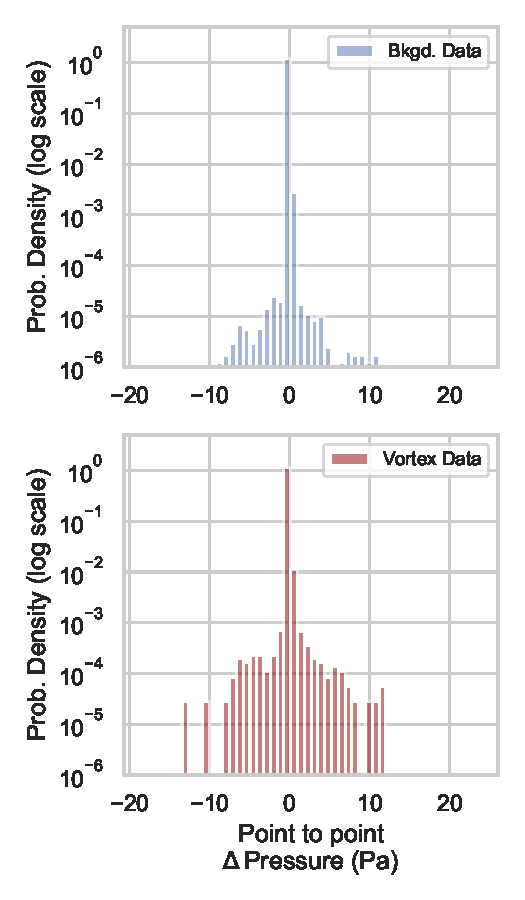
\includegraphics[width=0.45\textwidth]{figures/manuscript_static_detector_without_ma500_subtraction_overview_fig_v1.pdf}
    \caption{Statistical distributions of background and vortex data without any background subtraction applied before the point to point differences are calculated.}
    \label{fig_appendix:vortex_press_diff_without_bkgd_subtraction_dist_fit}
\end{figure}

\subsection{Full List of Event Detections}

\subsection{Example Calculation}

\begin{figure}
    \centering
    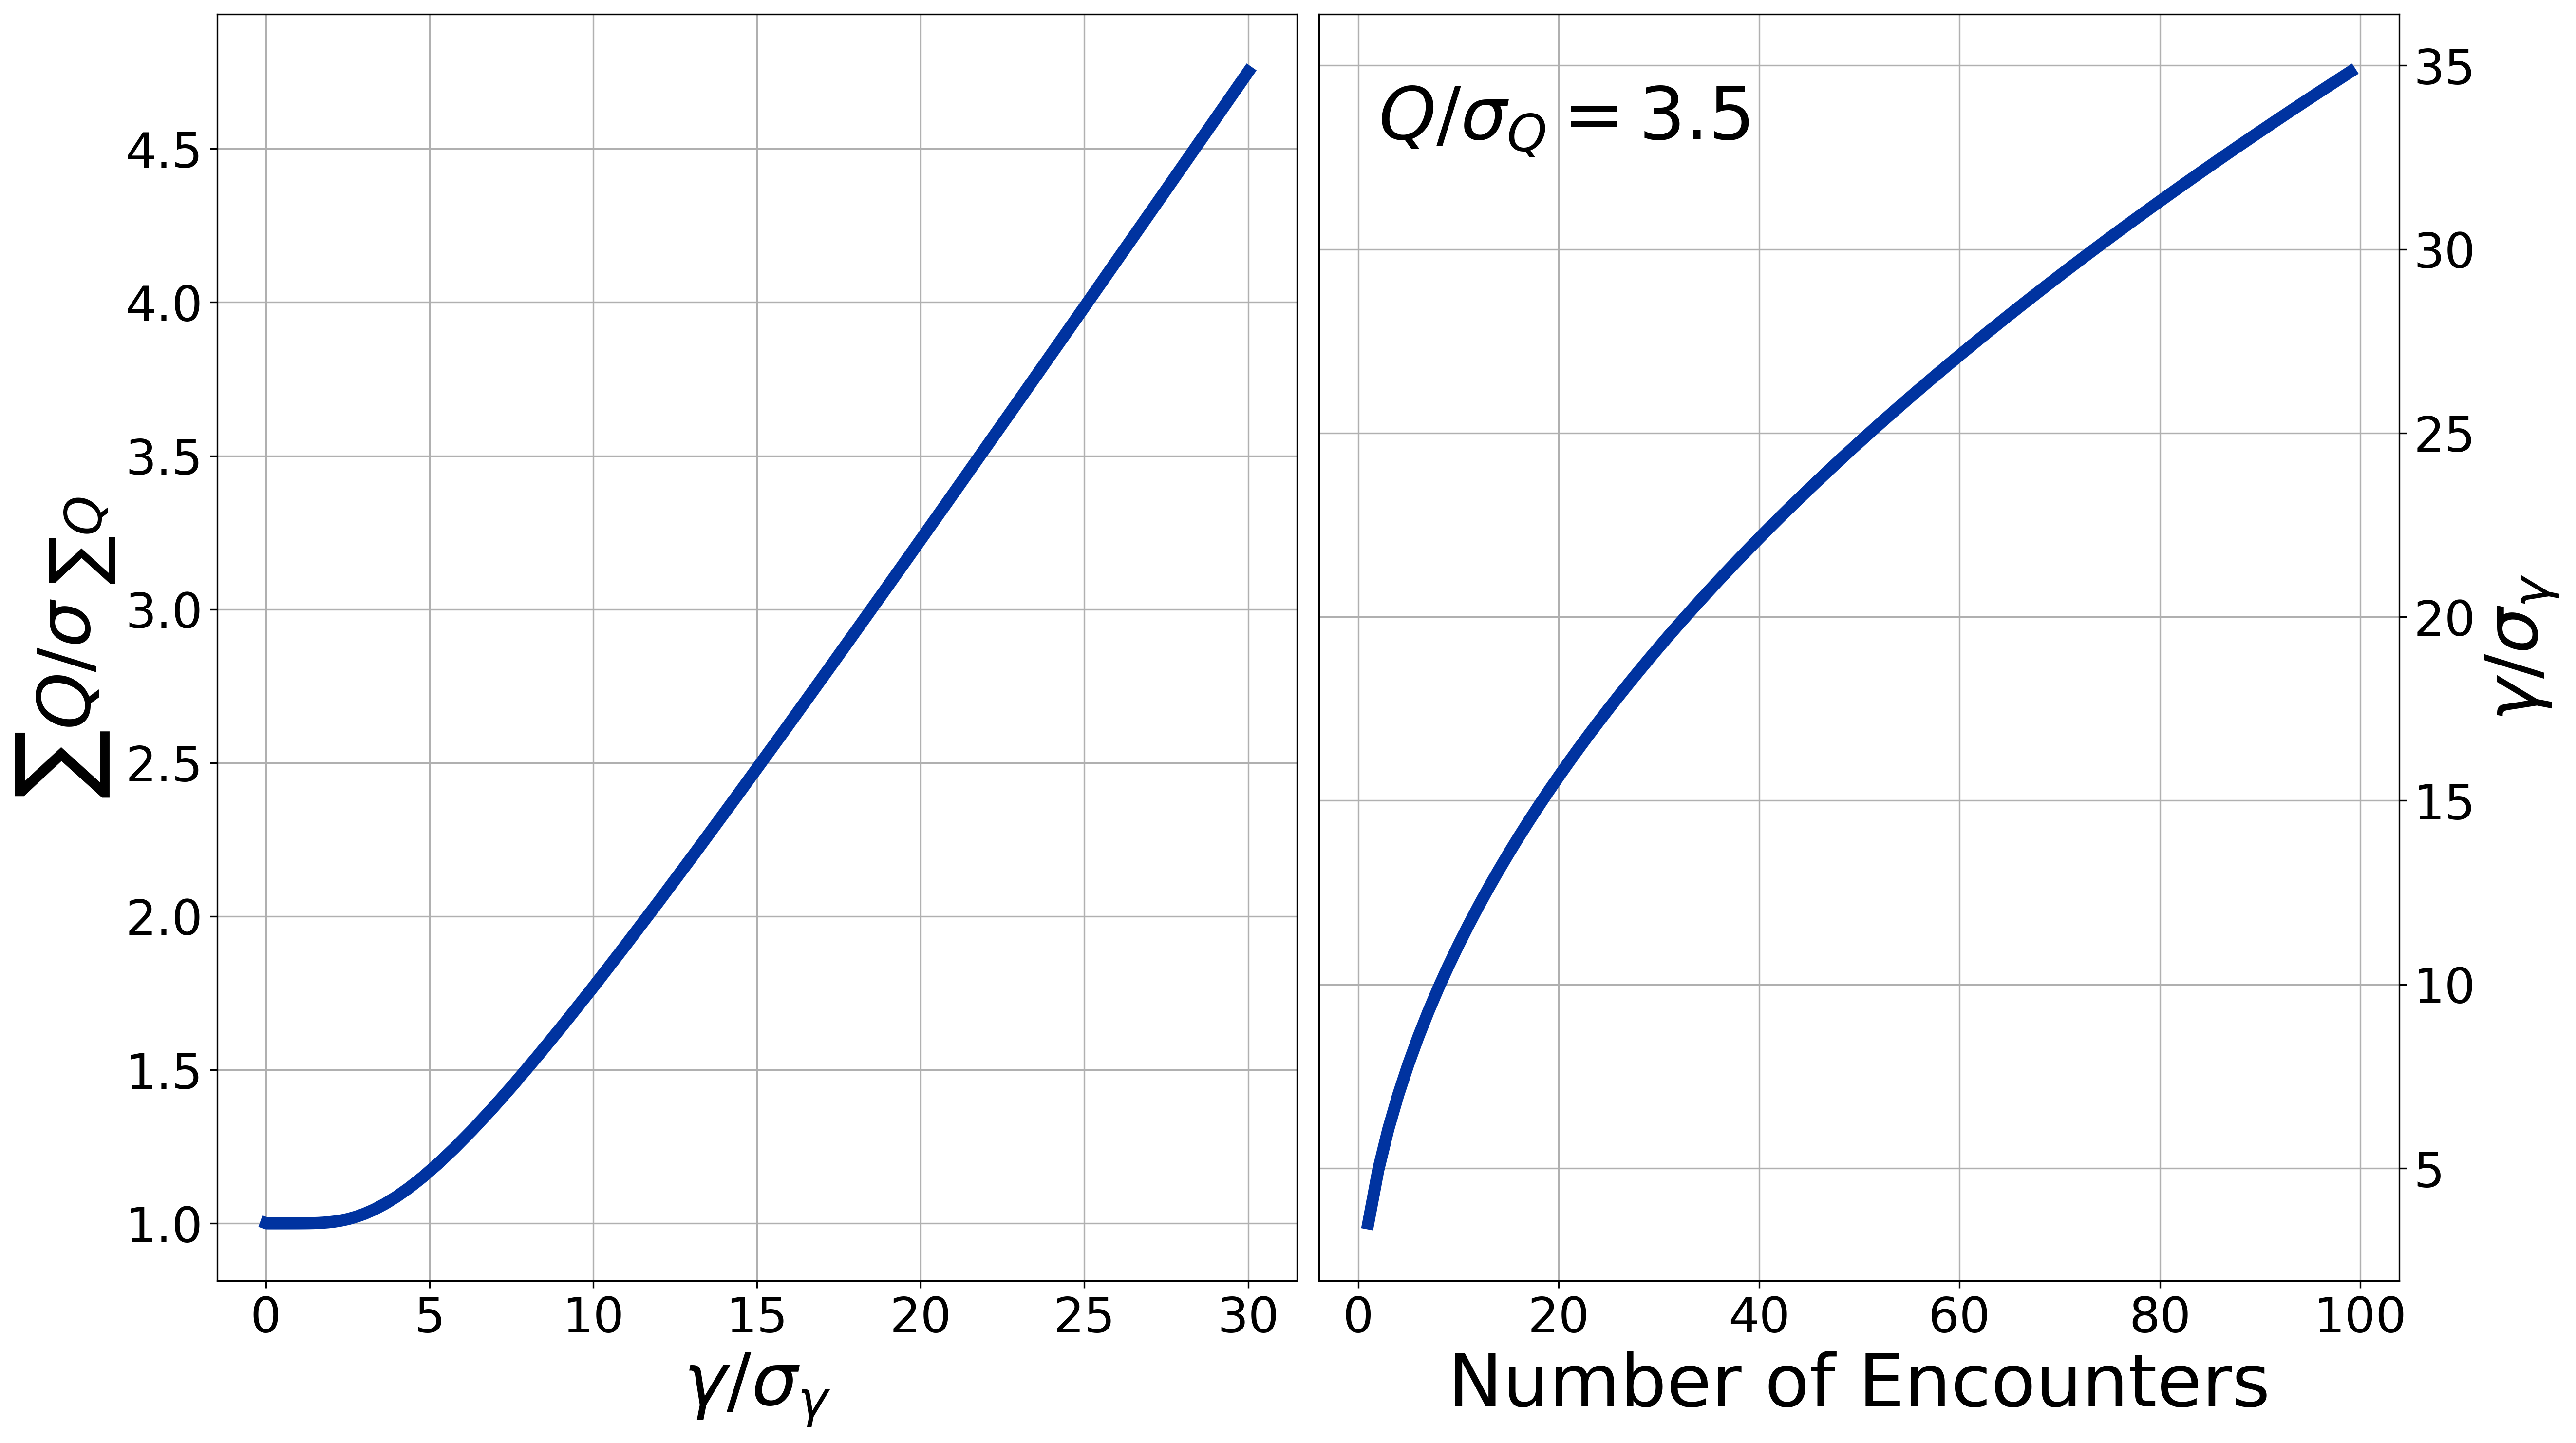
\includegraphics[width=\textwidth]{figures/Population_Weighted_Dust_Flux.png}
    \caption{(Left) How the relative uncertainty on the population-weighted dust flux $\sum Q$ depends on the relative uncertainty in the $\Delta P_{\rm c}$ relationship power-law index $\gamma$. (Right) How the relative uncertainty in $\gamma$ depends on the total number of dust devil encounters for our survey, assuming the dust flux for each encounter is estimated to about $3.5\sigma_Q$ precision.}
    \label{fig:Population_Weighted_Dust_Flux}
\end{figure}

Results from \cite{Neakreas2010} suggest the dust flux from a dust devil $Q \propto \Delta P_{\rm c}^\gamma$ with $\gamma = 3.4 \pm 0.73$, i.e. $\gamma/\sigma_\gamma = 4.7$, with $\Delta P_{\rm c}$ the pressure excursion at the center of the dust devil. How does that uncertainty on $\gamma$ impact our uncertainty on the total dust flux for a population of martian dust devils, and how much can we improve upon that estimate with our work? Martian dust devils are thought to have $\Delta P_{\rm c}$ values roughly distributed according to $\Delta P_{\rm c}^{-2}$ \cite{2016SSRv..203..277L}, i.e., the smaller $\Delta P_{\rm c}$ values are much more common than the larger ones. We can sum up the dust flux from such a population $\sum Q$ and estimate the uncertainty $\sigma_{\sum Q}$ that arises from the uncertainty on $\gamma$, as shown in the left panel of Figure \ref{fig:Population_Weighted_Dust_Flux}. For the results from \cite{Neakreas2010}, $\gamma/\sigma_\gamma = 4.7$, and the left panel of Figure \ref{fig:Population_Weighted_Dust_Flux} shows this means $\sum Q/\sigma_{\sum Q} \sim 1$, i.e., the population-weighted dust flux for martian dust devils is almost entirely unconstrained, at least based on that scaling relationship. But Figure \ref{fig:Population_Weighted_Dust_Flux} shows that increasing $\gamma/\sigma_\gamma$ even by a little bit pays substantial dividends in reducing the flux uncertainties. 

\begin{figure}
    \centering
    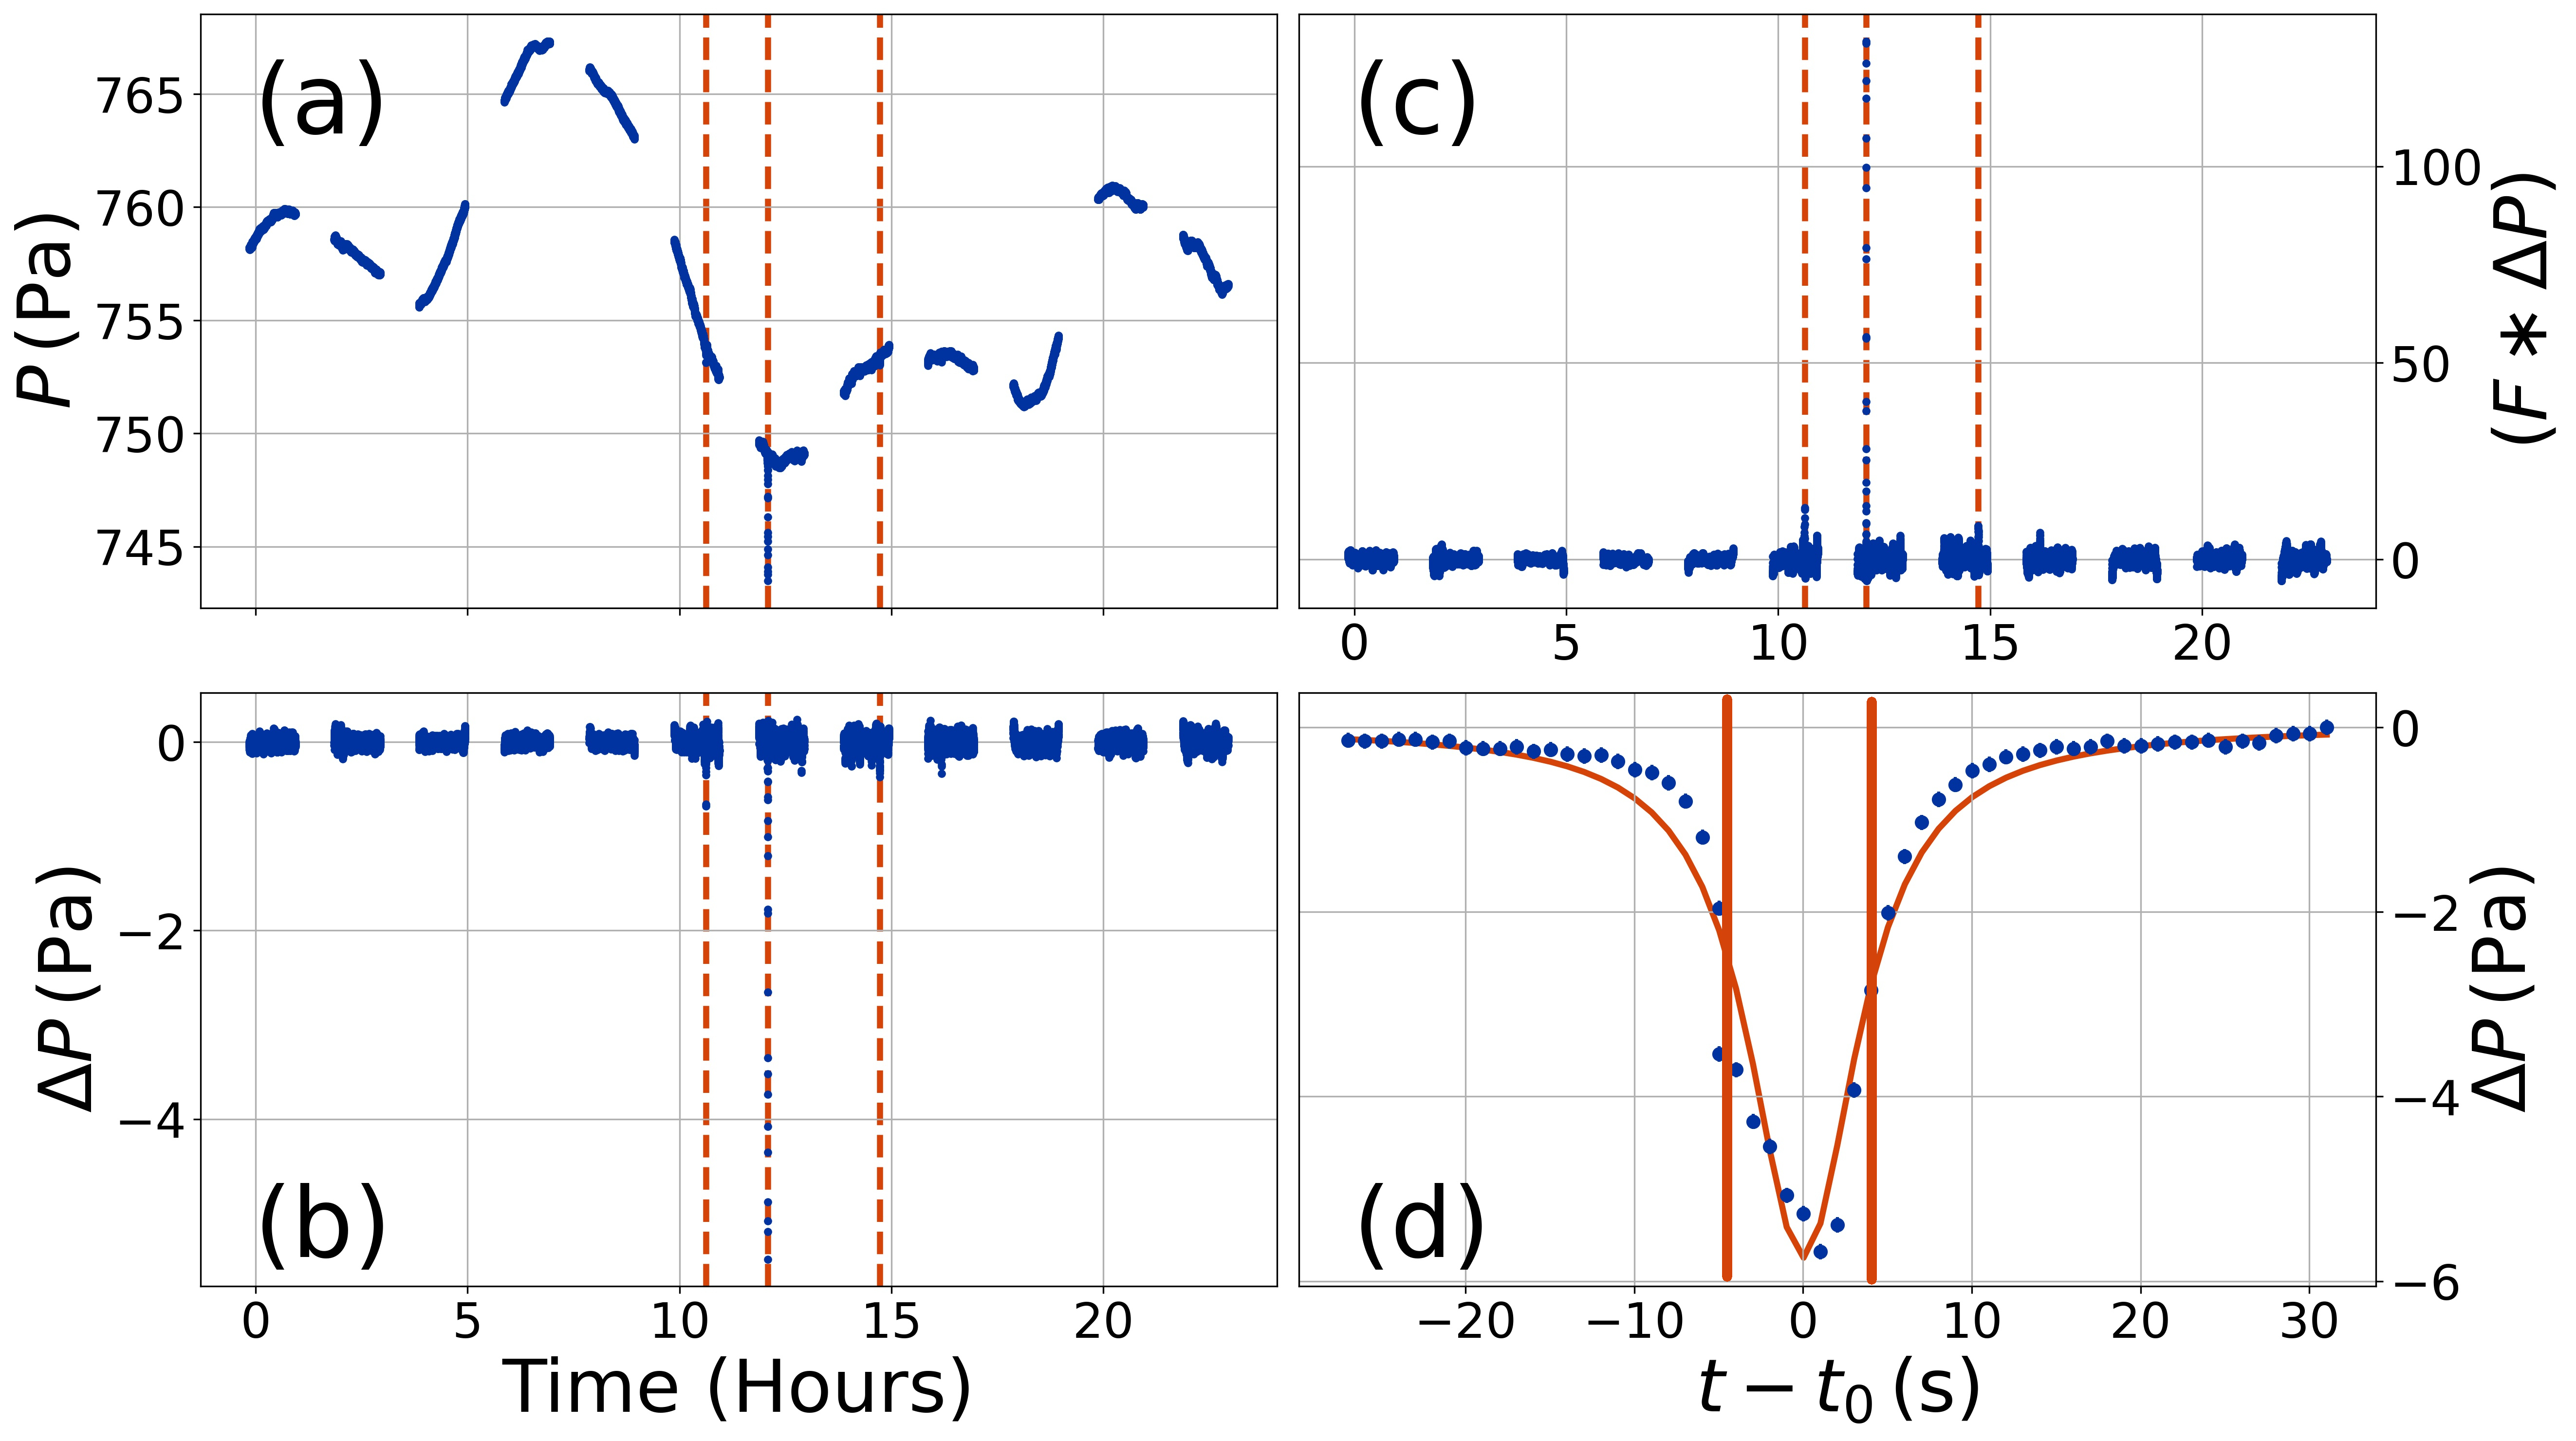
\includegraphics[width=\textwidth]{figures/conditioned_data_sol82.png}
    \caption{(a) The pressure time-series for sol 395, as blue dots. The vertical orange lines highlight the detected vortex signals. (b) The time-series after application of the mean boxcar filter. Apparent by eye, the scatter in the time-series increases around mid-day. (c) Convolution of the matched filter with the time-series in (b). The horizontal dashed orange line shows the detection threshold of 5. (d) A model fit (solid orange line) to the deepest vortex discovered on sol 395, along with the model fit parameters -- each point's uncertainty is calculated via $1.4826\ \times$ the median absolute deviation in the window centered on that point. The vertical orange lines show the full-width/half-max (FWHM) for this encounter.}
    \label{fig:data_conditioning_and_fit}
\end{figure}

Consider a vortex encounter like the one depicted in Figure \ref{fig:data_conditioning_and_fit}(d). As an initial simplified approach, we will assume that, if pressure time-series data are collected during the full-width/half-max (FWHM) of a vortex encounter (shown as the vertical orange lines in Figure \ref{fig:data_conditioning_and_fit}d), the vortex is recovered. From this standpoint, all vortices that pass near the sensor will be recovered if the sensor sampling rate is at least as large as $1/\Gamma_{\rm obs}$ for the shortest-duration vortex encounter. Based on the survey in \citet{2022PSJ.....3...20J}, a reasonable estimate for this shortest-duration encounter is $\Gamma_{\rm obs} = 1\,{\rm s}$, which suggests a sampling rate of at least $1\,{\rm Hz}$ as a minimum rate for recovering all encounters. Such a sampling rate has been typical for meteorological instrumentation deployed on the martian surface \citep[e.g.,][]{Spiga2021}, so for the illustrative calculation outlined here, let's assume that sampling rate, which means we expect to produce an estimate for $\Delta P_{\rm c}$ for each encountered vortex (although, N.B., this estimate will likely always fall below the actual $\Delta P_{\rm c}$ -- more later). Combining that assumption with the results shown in Figure \ref{fig:Population_Weighted_Dust_Flux}, how does running the pressure sensor for a given duration translate into an uncertainty on the dust flux estimate?

\begin{figure}
    \centering
    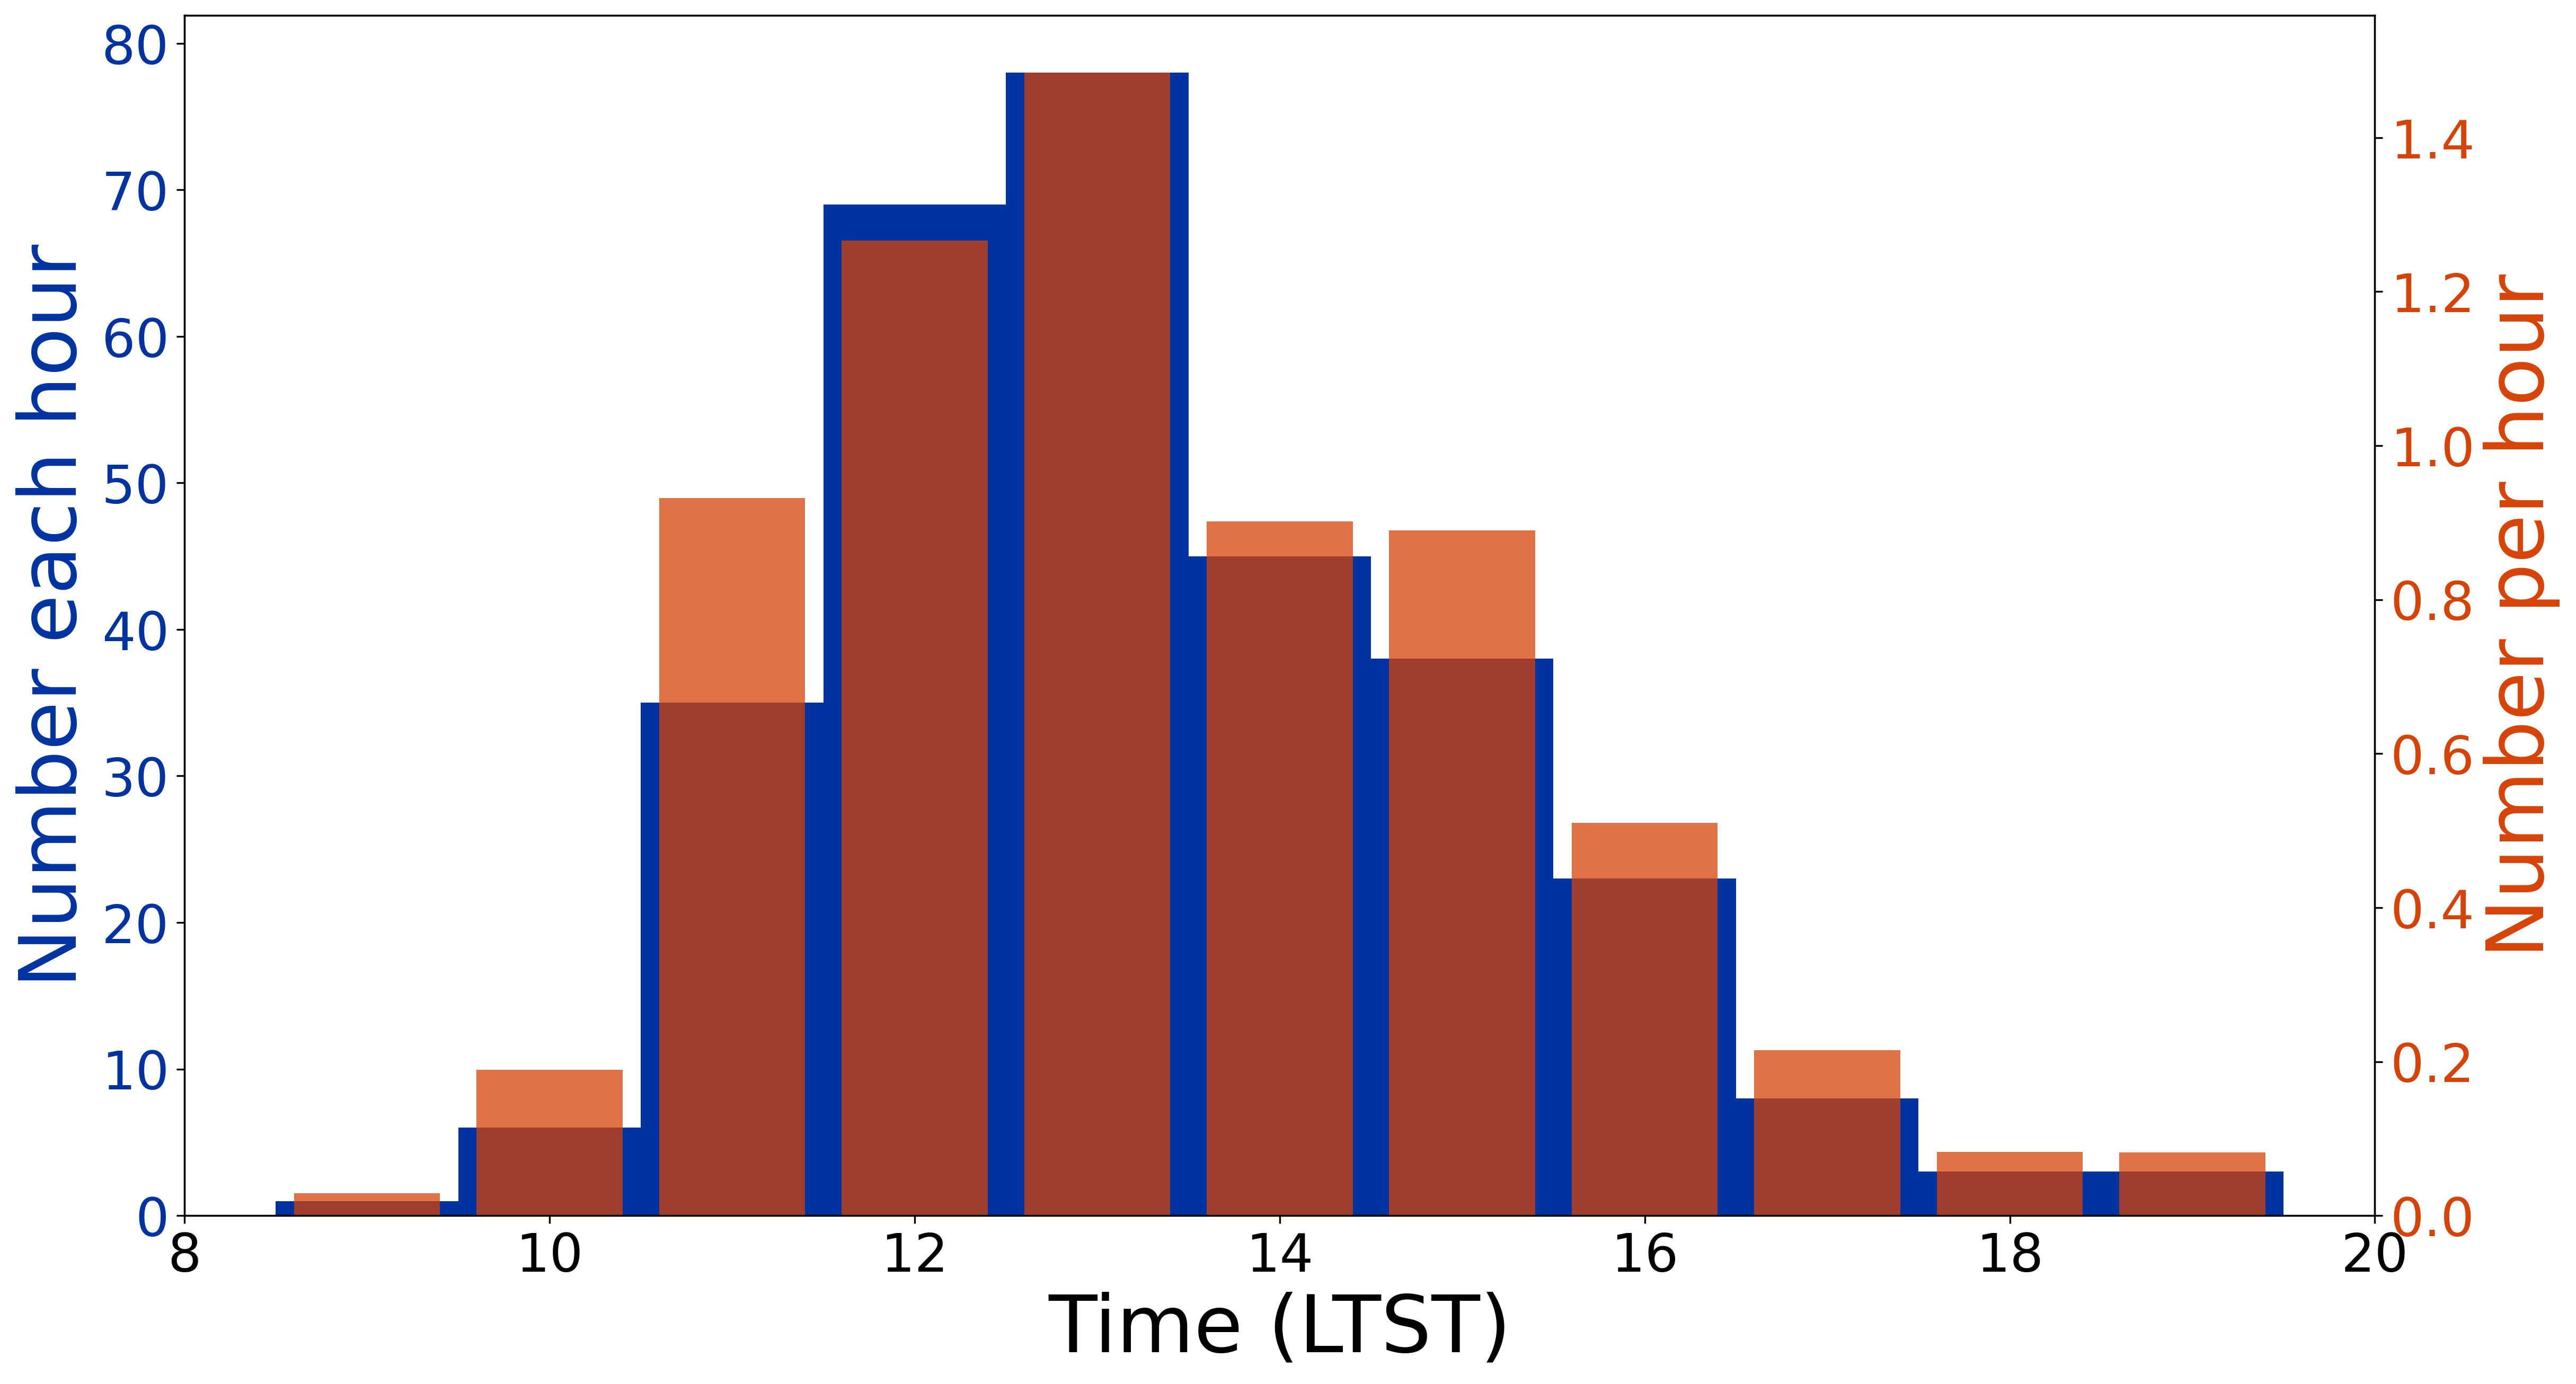
\includegraphics[width=\textwidth]{figures/vortex_occurrence_each_hour.png}
    \caption{The blue bars show the total number of vortex encounters that took place during that hour over the whole 89 sol dataset, while the orange bars show that number divided by the total number of hours during that period each sol observed throughout the 89 sol dataset. From \citet{2022PSJ.....3...20J}.}
    \label{fig:vortex_occurrence_each_hour}
\end{figure}

\citet{Jackson2022} found that, near mid-day on Mars, Mars 2020 saw about 1 vortex encounter per hour (Figure \ref{fig:vortex_occurrence_each_hour}). If, for simplicity, we imagine the pressure sensor ran at 1 Hz for an hour each sol during the mid-day period, we would expect to recover 40 vortex encounters after 40 sols, which allow us to estimate $\gamma/\sigma_\gamma \sim 20$, sufficient to estimate $\Sigma Q$ to about 3$\sigma$ precision (Figure \ref{fig:Population_Weighted_Dust_Flux}).